\documentclass[a4paper]{report}

% \usepackage[utf8]{inputenc}
% \usepackage[T1]{fontenc}
% \usepackage{textcomp}
\usepackage[english]{babel}
\usepackage{amsmath, amssymb}
\usepackage[separate-uncertainty=true, multi-part-units=single]{siunitx}
\usepackage[]{subfig}
\usepackage[colorlinks=true, anchorcolor=blue, linkcolor=blue, citecolor=blue, bookmarks=false,hyperfootnotes=false]{hyperref}
\usepackage[margin=1in]{geometry}
\usepackage{color,soul}
\usepackage{tabularx}

% figure support
\usepackage{import}
\usepackage{xifthen}
\pdfminorversion=7
\usepackage{pdfpages}
\usepackage{transparent}
\usepackage{physics}
\graphicspath{ {./figures/} }
% \setlength{\parindent}{0pt}
\usepackage{chngcntr}
\usepackage{verbatim}
\usepackage{indentfirst}
\numberwithin{equation}{section}
\counterwithin{figure}{section}
\newcommand{\incfig}[1]{%
		\def\svgwidth{\columnwidth}
		\import{./figures/}{#1.pdf_tex}

}

\pdfsuppresswarningpagegroup=1

% for citations / references
\usepackage[style=ieee]{biblatex}
\addbibresource{styx-report.bib}

\begin{document}

%----------------------------------------------------------------------------------------
%	TITLE PAGE
%----------------------------------------------------------------------------------------
\begin{titlepage} % Suppresses displaying the page number on the title page and the subsequent page counts as page 1
	\newcommand{\HRule}{\rule{\linewidth}{0.5mm}} % Defines a new command for horizontal lines, change thickness here
	
	\center % Centre everything on the page
	%------------------------------------------------
	%	Headings
	%------------------------------------------------
	
	\textsc{\LARGE Rheinische Friedrich-Wilhelms-Universit\"at Bonn }\\[4cm] % Main heading such as the name of your university/college
	
	\textsc{\Large Advanced Laboratory Course}\\[0.5cm] % Major heading such as course name
	
	\textsc{\large Performed on: May 12 - 13, 2022}\\[0.5cm] % Minor heading such as course title

	\textsc{\large Submitted on: June 20, 2022}\\[0.5cm] % Minor heading such as course title
	
	%------------------------------------------------
	%	Title
	%------------------------------------------------
	
	\HRule\\[0.4cm]
	
	{\huge\bfseries E217: STYX}\\[0.4cm] % Title of your document
	
	\HRule\\[1.5cm]
	
	%------------------------------------------------
	%	Author(s)
	%------------------------------------------------
	
	\begin{minipage}{0.4\textwidth}
		\begin{flushleft}
			\large
			\textit{Authors}\\
			Paarth Thakkar \\
			Keito Watanabe
		\end{flushleft}
	\end{minipage}
	~
	\begin{minipage}{0.4\textwidth}
		\begin{flushright}
			\large
			\textit{Tutor(s)}\\
			Patrick Bauer
		\end{flushright}
	\end{minipage}

	\vspace*{5em}

	\begin{minipage}{0.8\textwidth}
		\begin{centering}
			% \large
			\textbf{Abstract}\\[0.2cm]
            
		\end{centering}
	\end{minipage}
	
	% If you don't want a supervisor, uncomment the two lines below and comment the code above
	%{\large\textit{Author}}\\
	%John \textsc{Smith} % Your name
	
	%------------------------------------------------
	%	Date
	%------------------------------------------------
	
	%\vfill\vfill\vfill % Position the date 3/4 down the remaining page
	% \vfill\vfill
	
	% {\large\today} % Date, change the \today to a set date if you want to be precise
	
	%------------------------------------------------
	%	Logo
	%------------------------------------------------
	
	%\vfill\vfill
	%\includegraphics[width=0.2\textwidth]{placeholder.jpg}\\[1cm] % Include a department/university logo - this will require the graphicx package
	 
	%----------------------------------------------------------------------------------------
	
	% \vfill % Push the date up 1/4 of the remaining page
	
\end{titlepage}



\tableofcontents

\chapter{Introduction}



\chapter{Theory}

\section{Cosmic Rays}



Primary cosmic rays are highly energetic charged particles or nuclei with a long lifetime of order $10^6$ years or longer that are accelerated by 
astrophysical origins. These particles mainly consist of protons (85\%), but also consist of heavier nuclei such as Helium \cite{Tanabashi2018}. 
These cosmic rays propagate through intergalactic and interstellar space, losing energy through radiative processes \cite{DeDomenico2012}.
They are then captured by the Earth's magnetic field before arriving at Earth's atmosphere with energies ranging from MeV to GeV ranges. 
They then interact with the atmospheric nuclei on Earth, producing "secondaries", that is, particles produced from such interactions. The secondaries
produced are mainly pions ($\pi^\pm, \pi^0$), whereas kaons ($K^\pm, K^0, \bar{K}^0$) are only produced with a probability of 10\% compared to pions \cite{Grupen2005}. \par 

\begin{figure*}[!h]
	\centering
	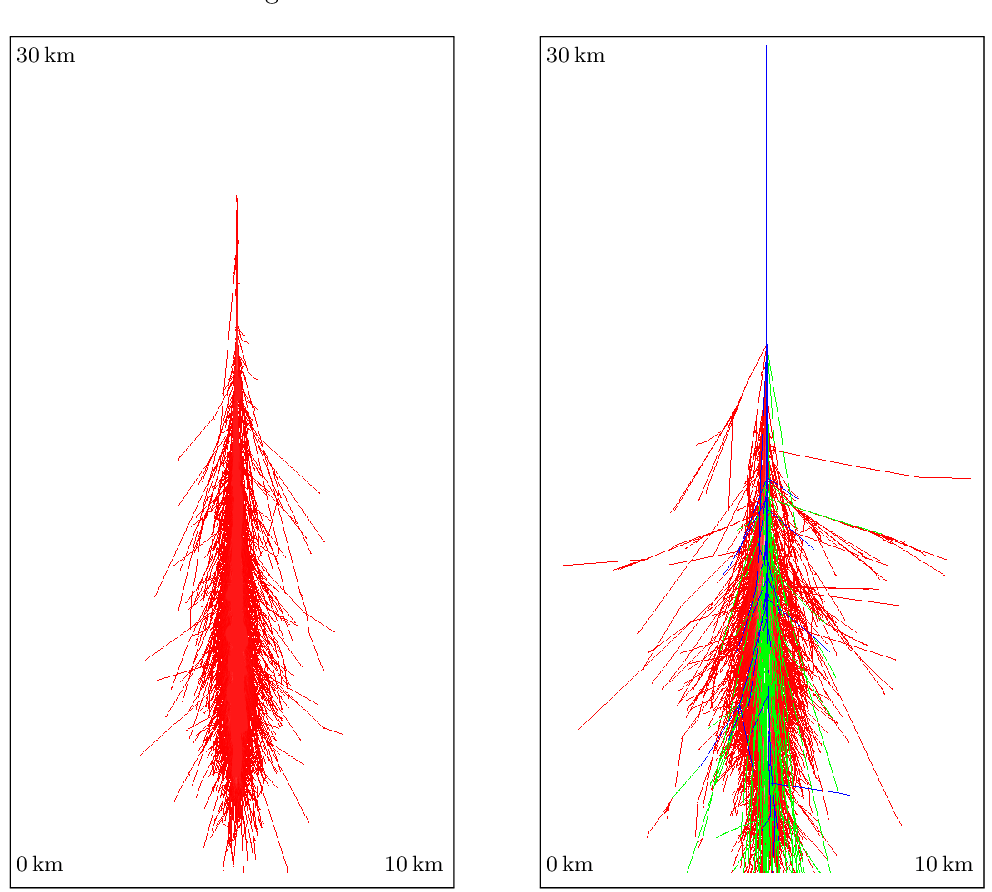
\includegraphics[width=0.6\textwidth]{em_hadronic_showers.png}
	\caption{ \textit{Left:} An electromagnetic shower induced by $\gamma$ at $\SI{1}{\tera\electronvolt}$. 
				\textit{Right: } A hadronic shower induced by a $\SI{1}{\tera\electronvolt}$ proton. Both plots show the lateral
				development of the showers at different altitudes. The red lines indicate electromagnetic components, blue indicates 
				hadronic components, and green indicate muon components (consisting of $\mu, \nu_\mu$) \cite{Haeffner2014}. }
	\label{fig:em_had_showers}
\end{figure*}

As pions and kaons are not stable, they decay into subsequent particles through various channels.  
The neutral pion most commonly decay into a pair of photons ($\pi^0 \rightarrow \gamma + \gamma$), which subsequently produces a pair of electron and positron (pair production). They then undergo 
subsequent annihilation and bremsstrahlung processes, creating an electromagnetic cascade consisting of these three particles. Charged 
pions and kaons, however, primarily decay into a pair of muon and its corresponding neutrino or anti-neutrino ($\pi^+, K^+ \rightarrow \mu^+ + \nu_\mu$, $\pi^-, 
K^- \rightarrow \mu^- + \bar{\nu}_\mu$). These muons can also decay weakly into electrons, which then create subsequent electromagnetic cascades.
At higher energies of $E > \SI{10}{\giga\electronvolt}$, these pions and kaons can also decay into subsequent pions, which 
creates a hadronic cascade primarily consisting of these particles. Fig. \ref{fig:em_had_showers} shows an example of an electromagnetic and hadronic cascade that occurs from cosmic rays.



Through such electromagnetic and hadronic cascades, most charged particles are absorbed by the atmosphere and thus do not reach sea level. However, most of the muons 
produced from pions and kaons reach sea level due to their long lifetime, and as such approximately 80\% of the charged particles that reach sea level are muons.
The flux of muons detected at sea level is approximately 1 particle per cm$^2$ per minute, and as such one can detect more than $7 \times 10^{6}$ muons for an 
overnight measurement with a detector with an area of $\SI{1}{\meter\squared}$.  Neutrinos also reach sea level as they only interact weakly with matter and has a 
low interaction probability \cite{Grupen2005}. In the setup of our experiment, however, we are not able to detect neutrinos and thus only muons are detected. 
Fig. \ref{fig:air_shower} shows the schematic of a typical air shower from a primary cosmic ray. \par 


\begin{figure*}[!h]
	\centering
	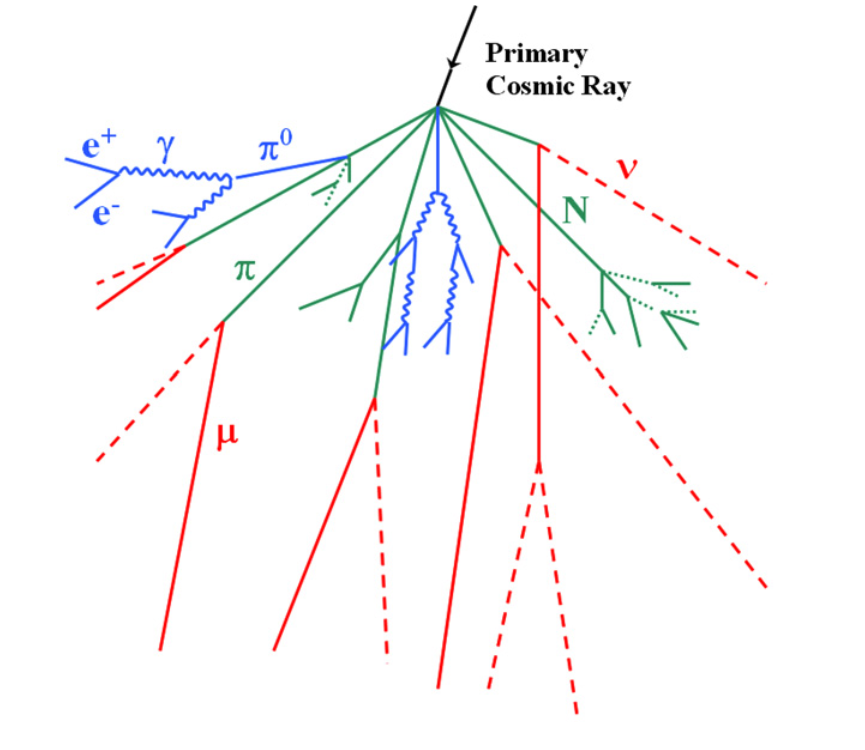
\includegraphics[width=0.6\textwidth]{air_shower.png}
	\caption{A typical air shower resulting from interaction of primary cosmic ray with the atmosphere. Electromagnetic cascades are shown in blue and hadronic 
	cascades are shown in green. The muons and neutrinos (indicated in red) produced from pion and kaon decays are the most common particles that reach sea level 
	\cite{Blanco2009}.}
	\label{fig:air_shower}	
\end{figure*}

The total muon intensity distribution depends on the zenith angle $\theta$, i.e. the angle from the local zenith of the location of 
measurement. Such dependence is due to the stronger absorption of muons as they have to propagate through larger distances at 
inclined angles. The intensity distribution is given as such: 
\begin{equation}
    I(\theta) = I_0 \cos^n \theta 
\end{equation}
where $I_0$ is the intensity at the local zenith $\theta = 0^\circ$ \cite{Grupen2005}. The exponent of the cosine function at 
sea level is $n = 2$ as most muons have energies $E_\mu \sim \SI{3}{\giga\electronvolt}$ when they reach sea level \cite{Stefano2012}.

\section{Gaseous Detectors}



\chapter{Experimental Setup}

fdaf


\printbibliography

\end{document}